\documentclass{article}

% Language setting
% Replace `english' with e.g. `spanish' to change the document language
%\usepackage[deutsch]{babel}

% Set page size and margins
% Replace `letterpaper' with `a4paper' for UK/EU standard size
\usepackage[letterpaper,top=2cm,bottom=2cm,left=3cm,right=3cm,marginparwidth=1.75cm]{geometry}

% Useful packages
\usepackage{amsmath}
\usepackage{graphicx}
\usepackage[colorlinks=true, allcolors=blue]{hyperref}
\usepackage{hhline}
\usepackage{tabularx}
\usepackage{float}

\title{Gleichrichter}
\author{Lukas Babitschew, Phil Gith, Stefan Ertl}

\begin{document}
\maketitle


\section{Versuchsziel}

Im folgenden Versuch werden mehrere Messungen an einem Einweggleichrichter und einem Gleichrichter in Graetzschaltung duchgeführt. Dabei sollen an bestimmten Messpunkten Gleich- und Wechselanteile der Schaltungen gemessen werden und dadurch die Funktionsweise und Limitation eines Gleichrichters dargestellt werden 

\section{Versuchsaufbau}
\begin{figure}[H]
\centering
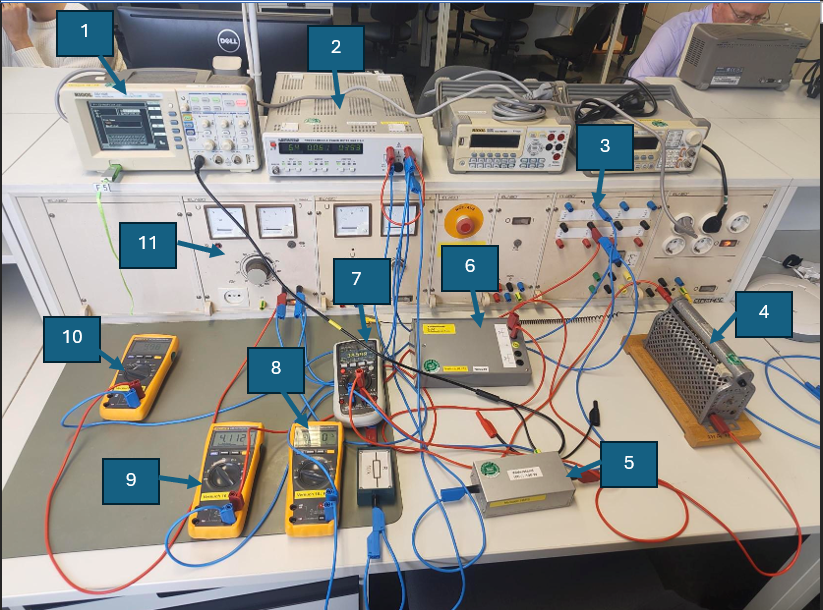
\includegraphics[width=0.75\linewidth]{Bild(4).png}
\caption{Versuchsaufbau Einweggleichrichter.}
\end{figure}

\begin{enumerate}
    \item Osziloskop
    \item Hameg Leistungsmessgerät
    \item Einweggleichrichter aus vier Dioden
    \item Einstellbarer Widerstand
    \item 100 $\Omega$
    \item Kondensatorparallelschaltung
    \item Strommessgerät
    \item Spannungsmessgerät
    \item Spannungsmessgerät
    \item Spannungsmessgerät
    \item Trenntransformator
    
\end{enumerate}

\begin{figure}[H]
\centering
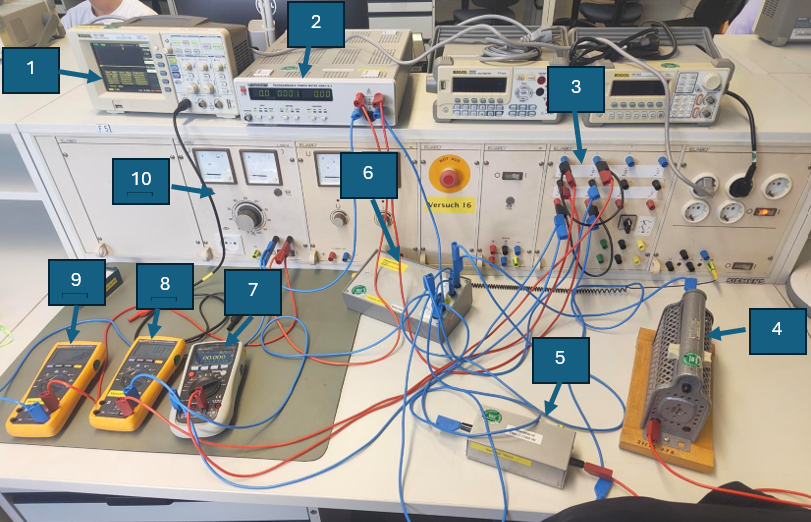
\includegraphics[width=0.75\linewidth]{Bild(3).png}
\caption{Versuchsaufbau Graetzschaltung}
\end{figure}

\begin{enumerate}
    \item Osziloskop
    \item Hameg Leistungsmessgerät
    \item Graetzschaltung aus vier Dioden
    \item Einstellbarer Widerstand
    \item 100 $\Omega$
    \item Kondensatorparallelschaltung
    \item Strommessgerät
    \item Spannungsmessgerät
    \item Spannungsmessgerät
    \item Trenntransformator
    
\end{enumerate}

\section{Versuche}
\subsection{Einweggleichrichter}
\begin{figure}[H]
\centering
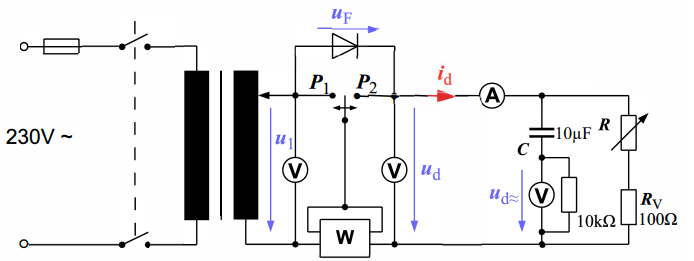
\includegraphics[width=0.75\linewidth]{Bildun.png}
\caption{Schaltbild Einweggleichrichter}
\end{figure}

Bei diesem Versuch wurde eine einzelne Diode verwendet, um ein Wechselsignal gleichzurichten. Hierzu lässt die Diode die positive Halbwelle durch, blockt aber die negative Halbwelle ab. Das dadurch entstandene Signal besitzt nun Gleich- und Wechselanteile.
\\\\
Folgende Messwerte haben sich für eine Eingangswechselspannung von 10 V ergeben.

\begin{table}[H]
\centering
\begin{tabular}{|l||l|l|l|}
\hline
 Größe &Arithmetischer Mittelwert &Effektivwert &Signalart\\ \hline
 $u_1$ (V) &0,37 &9,73 &Wechselgröße\\ \hline
 $u_d$ (V) &4,12 &6,47 &Mischgröße\\ \hline
 $u_d \approx$  (V) &-0,035 &4,63 &Wechselgröße\\ \hline
 $u_f$ (V) &4,15 &7,10 &Mischgröße\\ \hline
\end{tabular}
\caption{Messwerte}
\end{table}

Zum Vergleich wurden die selben Messwerte anhand der Daten des Osziloskopes nachberechnet.

\begin{table}[H]
\centering
\begin{tabular}{|l||l|l|l|}
\hline
 Größe &Arithmetischer Mittelwert &Effektivwert &Signalart\\ \hline
 $u_1$ (V) &0,36 &9,73 &Wechselgröße\\ \hline
 $u_d$ (V) &4,13 &6,49 &Mischgröße\\ \hline
 $u_d \approx$  (V) &0 &4,63 &Wechselgröße\\ \hline
 $u_f$ (V) &4,17 &7,13 &Mischgröße\\ \hline
 $i_d$ (mA) &39 &61,2 &Mischgröße\\ \hline
\end{tabular}
\caption{Berechnete Werte}
\end{table}

Der Strom $i_d$ kann über die Spannung $u_d$ und dem Widerstand im darauffolgenden Zweig bestimmt werden. Da der Widerstand des Kondensators und 10 k$\Omega$ Widerstandes deutlich höher ist der des einstellbaren Widerstandes und $R_v$, ist der Strom relativ akkurat bestimmbar mit \[i_d = \frac{U_rv}{•R_v}\]

Will man den Effektivwert der Mischgröße $u_d$ mit einem Digitalmultimeter bestimmen, muss man beachten, dass entweder Effektivwert des Gleichanteils oder Effektivwert des Wechselanteils gemessen werden kann. Folgende Werte wurden mit einem Fluke Messgerät bestimmt.

\[
	U_{1eff} = 10V;
\]
\[
	U_{deff}(DC) = 4,16; U_{deff}(AC) = 5,03
\]

Der tatsächliche Effektivwert ergibt sich aus
\[
	\sqrt{{U_{deff}(DC)}^2 + {U_{deff}(AC)}^2}
\]

Draus ergibt sich:
\[
	\sqrt{{(4,16\ V)}^2 + {(5,03\ V)}^2} = 6,53\ V
\]

Das Hameg Leistungsmessgerät dagegen berechnet automatisch den korrekten Effektivwert:

\[
	U_{1eff} = 9,9V
\]


\[
	U_{deff} = 6,4V
\]




\begin{figure}[H]
\centering
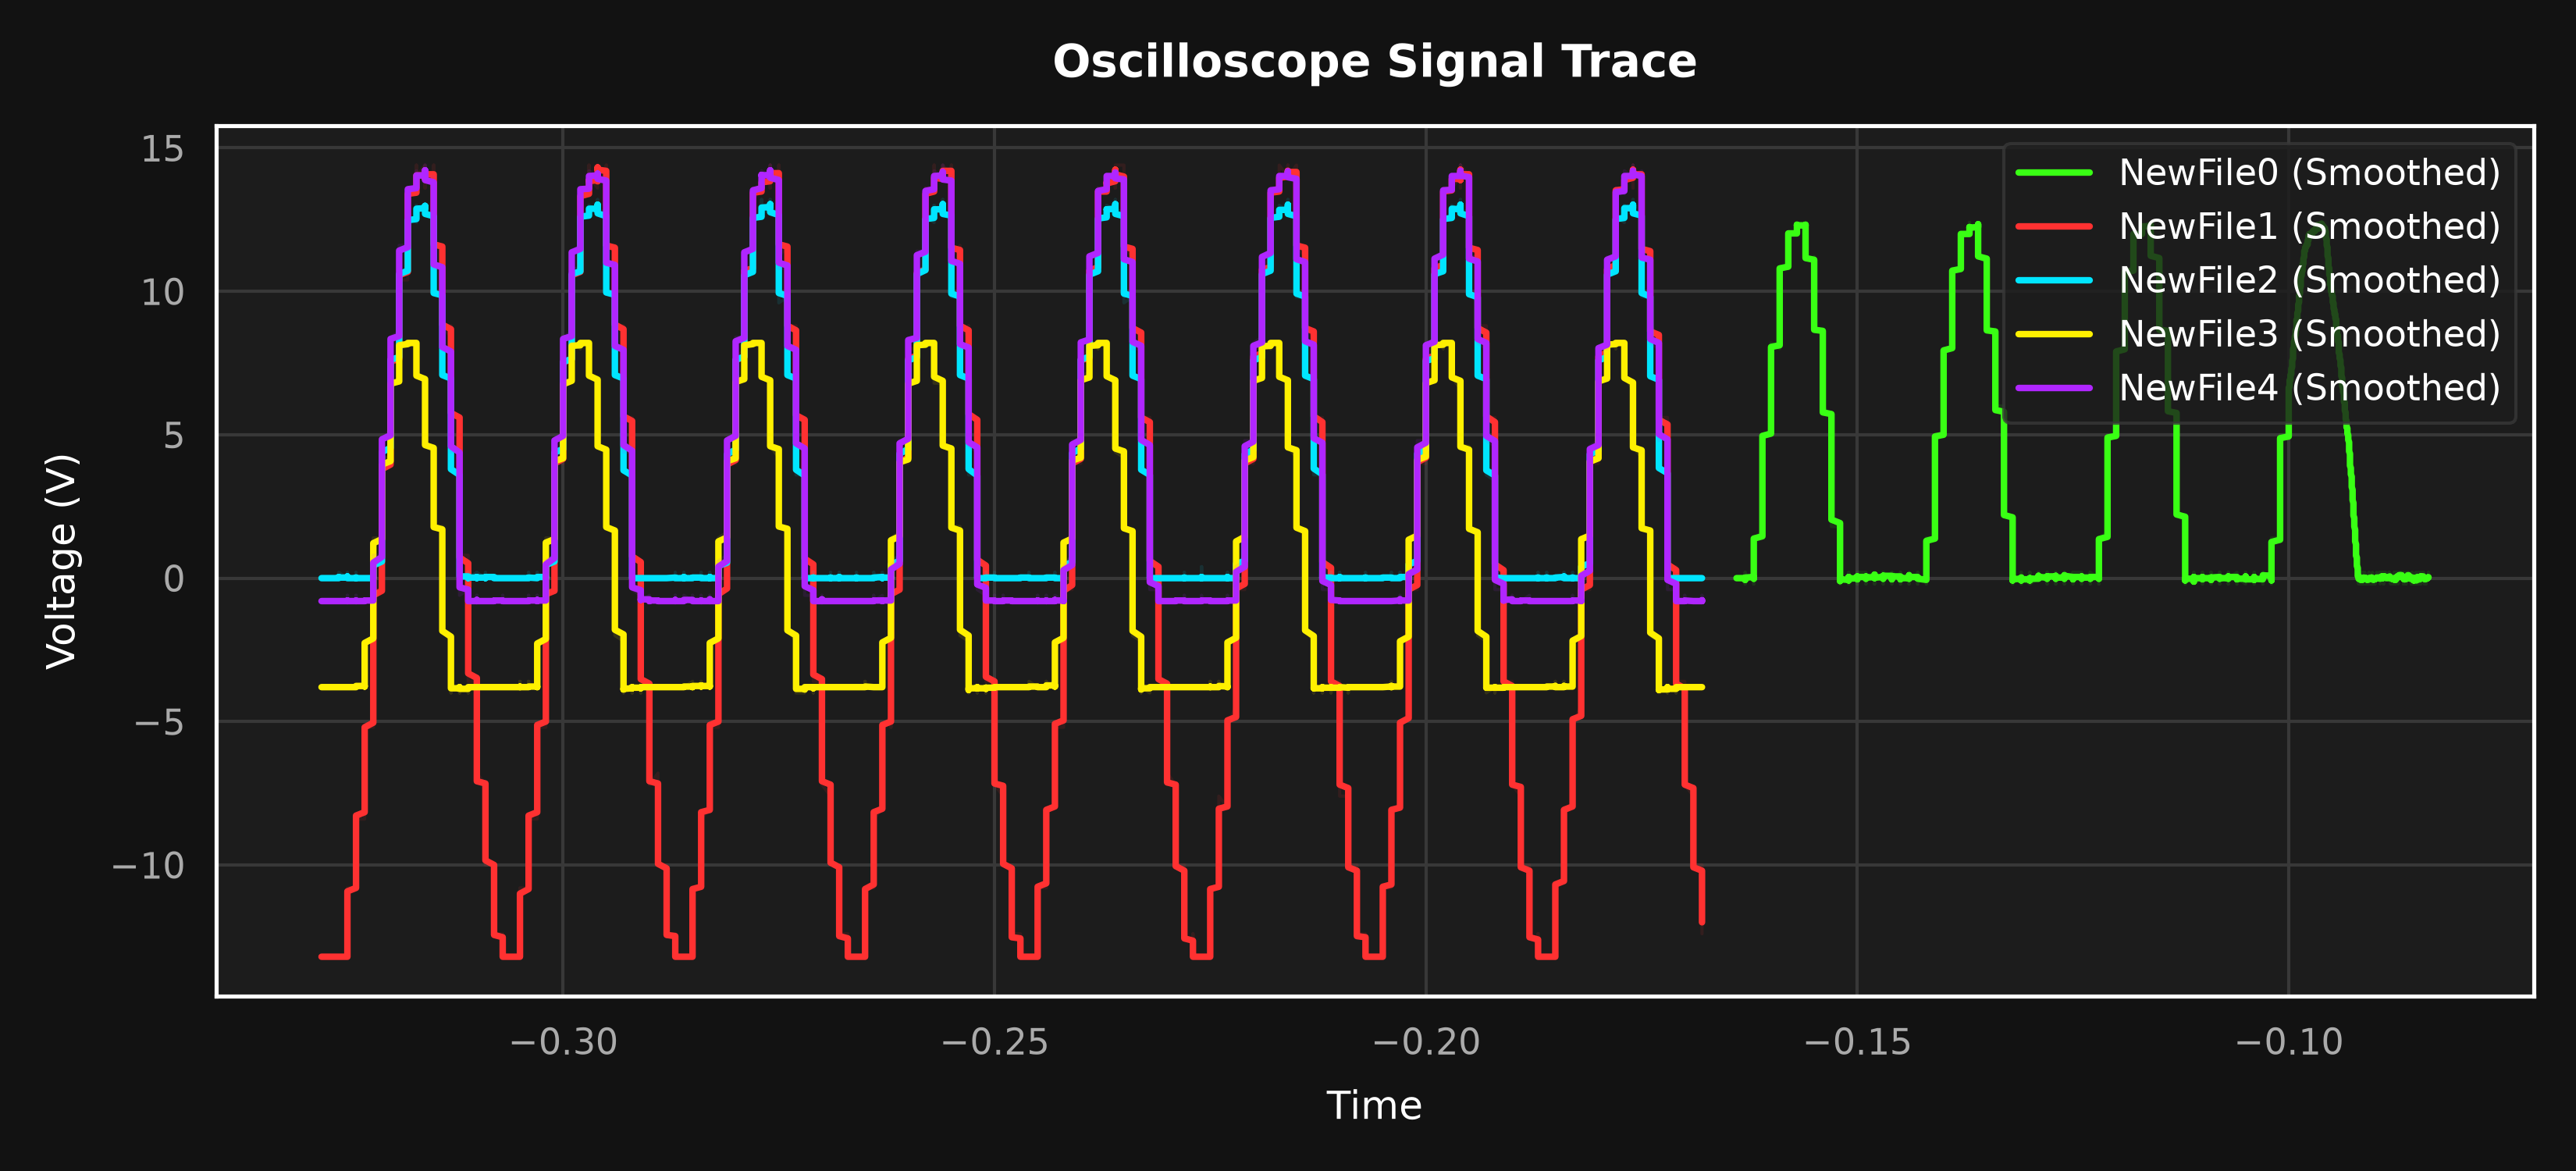
\includegraphics[width=1\linewidth]{41.png}
\caption{Schaltbild Einweggleichrichter}
\end{figure}

Die Diode lässt nur die positive Halbwelle der reinen Wechselspannung $u_1$ durch, der negative Teil fällt an der sperrenden Diode ab. Diese resultierende Welle besitzt deshalb nur noch die positiven Anteile des ursprünglichen Sinus mit der Amplitude $u_1 - 0,7/ V$, da die Durchlassspannung der Diode überwunden werden muss.
Demnach fällt der gesamte negative Teil and der Diode in $u_f$ ab. 
\[u_1 = u_d + u_f\]

Der Gleichanteil von $u_d$ wird anschließend von dem Kondensator herausgefiltert und verschiebt den Spannungsverlauf um 4 V nach unten ($u_{d \approx}$).

\subsubsection{i}


\end{document}